\begin{frame}{2-Punkt-Crossover}
    \begin{columns}[T] % T aligns the tops of the columns
        \begin{column}{0.65\textwidth}
            \vspace*{0.4cm}
            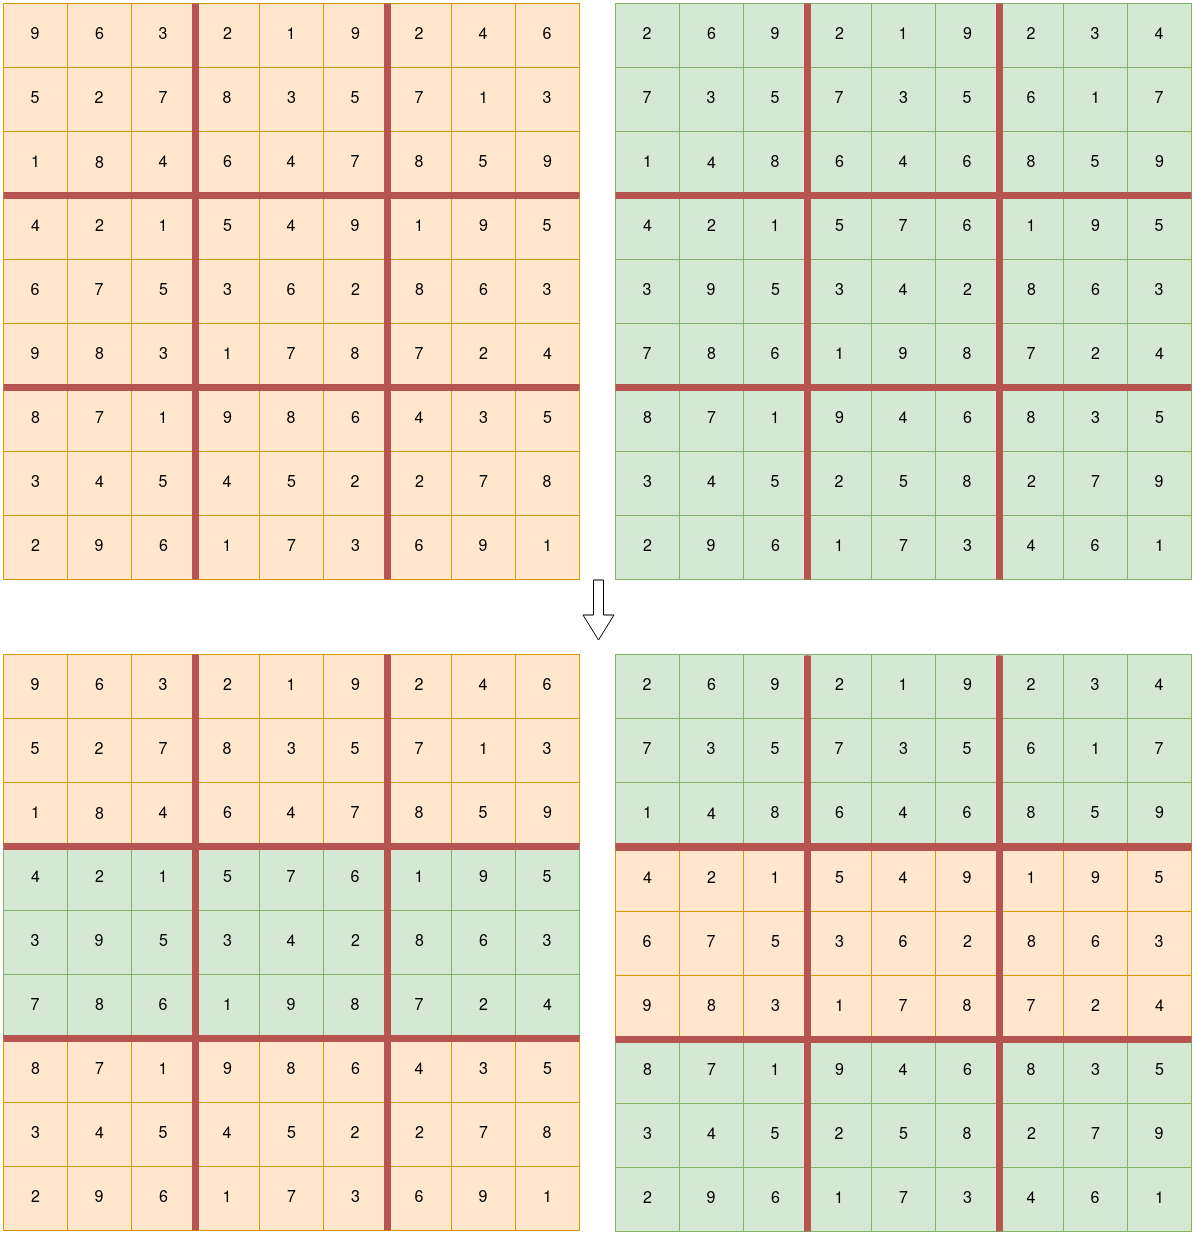
\includegraphics[width=\textwidth]{Pictures/2-Punkt-Crossover.png}
        \end{column}
        \begin{column}{0.35\textwidth}
            \begin{itemize}
                \vspace*{0.4cm}
                \item Invariante (keine Kollision in Blöcken) bleibt erhalten
                \item Übernahme der Eltern in neue Population
                \item "{}Auffüllen{}"{} der Population durch Crossover 
                \item Zeilenkollisionen bleiben erhalten
            \end{itemize}
        \end{column}
    \end{columns}
    \note[item]{Uebernahme selektierter Eltern}
    \note[item]{Auffuellen der Population durch Crossover}
    \note[item]{Ziehen ohne Zuruecklegen aus Liste von Eltern}
    \note[item]{Blockinvariante und Reihenkollisionen beliben erhalten}
\end{frame}
\begin{frame}{Diagonales-Crossover}
    \centering
    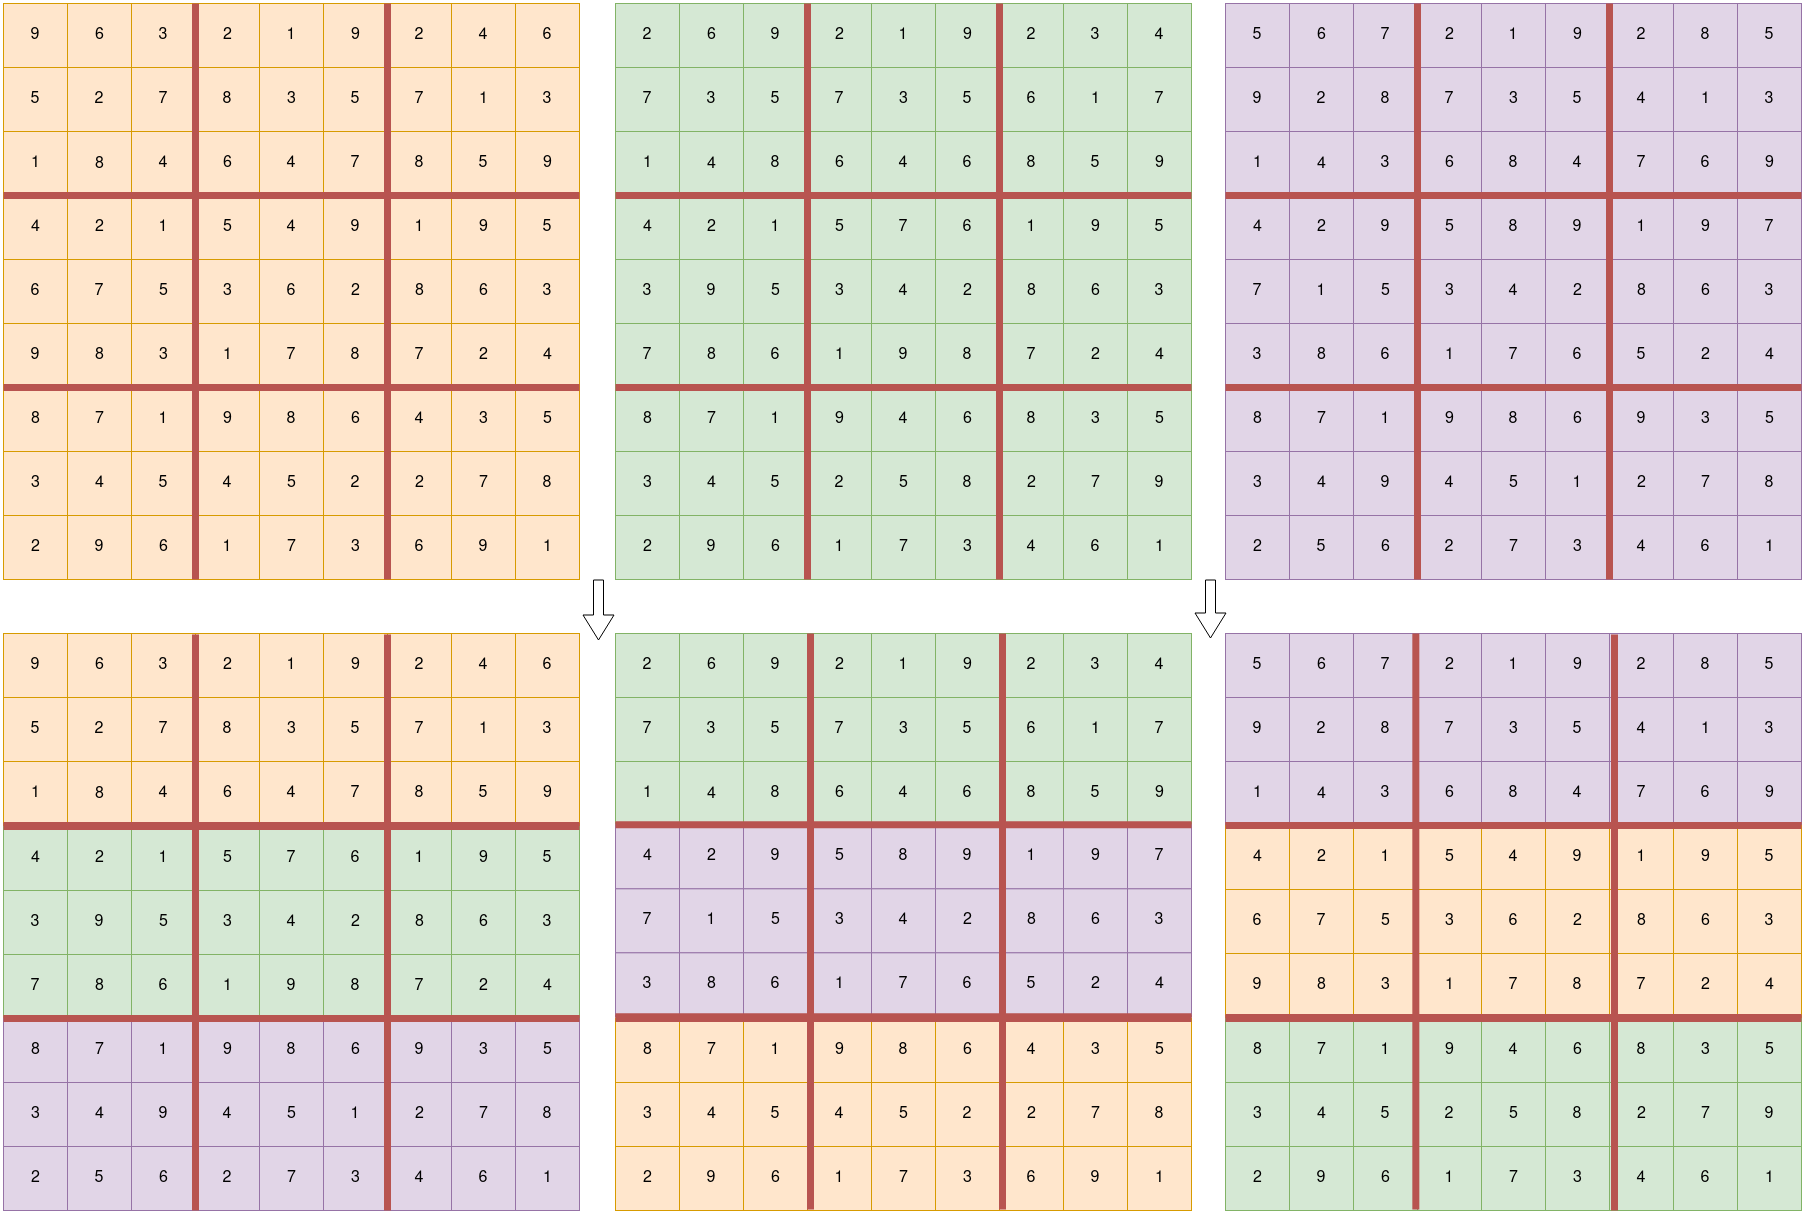
\includegraphics[width=\textwidth]{Pictures/Diagonales-Crossover.png}
\end{frame}